\documentclass[10pt]{article}
\usepackage[a4paper,margin=18mm]{geometry}
\usepackage{amsmath,amssymb,booktabs,array,enumitem}
\usepackage[T1]{fontenc}\usepackage{lmodern}
\usepackage{tikz}\usetikzlibrary{shapes.gates.logic.US,positioning,arrows.meta,patterns,calc}
\usepackage[hidelinks]{hyperref}
\setlength{\parindent}{0pt}\setlength{\parskip}{4pt}
\setlength{\emergencystretch}{2em}
\newcommand{\VDD}{V_{DD}}
\newcommand{\mos}[4]{\begin{scope}[shift={(#1,#2)}]
\draw (0,.24)--(0,-.24);\draw (0,.20)--(.25,.20)--(.25,.5);
\draw (0,-.20)--(.25,-.20)--(.25,-.5);\draw (-.16,.23)--(-.16,-.23);
\ifnum#4=1\draw (-.26,0) circle (.06);\draw (-.75,0)--(-.32,0);\else\draw (-.75,0)--(-.16,0);\fi
\node[anchor=east,font=\scriptsize] at (-.76,0) {$#3$};\end{scope}}
\newcommand{\ground}[2]{\draw (#1,#2)--(#1,{#2-.12});\draw ({#1-.17},{#2-.12})--({#1+.17},{#2-.12});\draw ({#1-.11},{#2-.20})--({#1+.11},{#2-.20});}
\newcommand{\rail}[3]{\draw (#1,#2)--(#1,{#2+.14});\node[above,font=\scriptsize] at (#1,{#2+.14}) {$#3$};}

\newcommand{\hmos}[4]{\begin{scope}[shift={(#1,#2)}]
\draw(-.24,0)--(.24,0);\draw(-.2,0)--(-.2,-.25)--(-.5,-.25);\draw(.2,0)--(.2,-.25)--(.5,-.25);
\draw(-.23,.16)--(.23,.16);
\ifnum#4=1\draw(0,.26)circle(.06);\draw(0,.32)--(0,.75);\else\draw(0,.16)--(0,.75);\fi
\node[below,font=\scriptsize]at(0,-.32){#3};\end{scope}}
\begin{document}\begin{center}{\large\bfseries EE3032 Introduction to VLSI Design -- Final}\end{center}
\textbf{Fall 2010.} All eight original questions; printed total of 130 points retained.
\textbf{1. (30 points)} Answer the following questions.
\begin{enumerate}[label=(\alph*),leftmargin=7mm,itemsep=1pt]
\item List two requirements for drawing the layout of a cell in the cell library. (4 points)
\item The dynamic power dissipation (switching power) of a complex gate can be divided two power components. List the two power components. (4 points)
\item List two design rules for avoiding glitch power of a CMOS circuit. (4 points)
\item List two approaches for coping with the power and ground bounce. (4 points)
\item List two major problems of the dynamic logic. (4 points)
\item List two limitations of the CMOS domino logic. (4 points)
\item What are the core-limited design and the pad-limited design? (4 points)
\item What is the physical design? (2 points)
\end{enumerate}
\textbf{2. (15 points)} Figure 1 shows a register realized by two low-cost latches. Complete the following questions.
\begin{enumerate}[label=(\alph*),leftmargin=7mm]
\item What type of the register is? Explain your answer. (5 points)
\item Assume that the switching threshold voltage of inverter Inv1 is $V_{dd}/2$ and the turn-on equivalent resistances of N1,N2,P1,P2 are $R_{N1},R_{N2},R_{P1},R_{P2}$, respectively. List two inequalities for determining the sizes of P2 and N2. (10 points)
\end{enumerate}
\begin{center}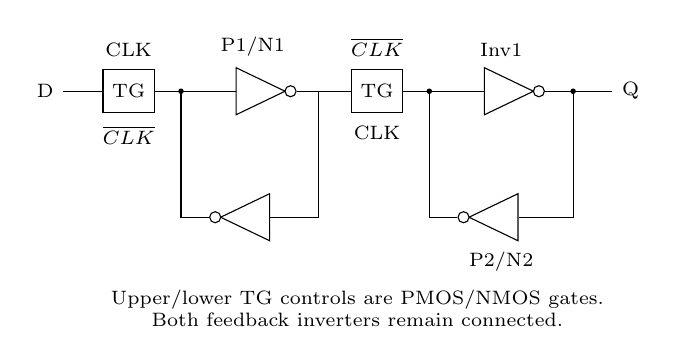
\begin{tikzpicture}[x=.83cm,y=.8cm,font=\scriptsize]
\node[draw,minimum width=.6cm,minimum height=.55cm](t1)at(.7,2.5){TG};\draw(-.3,2.5)node[left]{D}--(t1.west);\node[above]at(.7,2.9){CLK};\node[below]at(.7,2.1){$\overline{CLK}$};
\node[not gate US,draw,minimum width=.7cm](i1)at(2.6,2.5){};\draw(t1.east)--(i1.input);\node[above]at(2.6,2.9){P1/N1};\node[not gate US,draw,rotate=180,minimum width=.7cm](f1)at(2.6,.5){};\draw(i1.output)--(3.6,2.5)--(3.6,.5)--(f1.input);\draw(f1.output)--(1.5,.5)--(1.5,2.5);\fill(1.5,2.5)circle(1pt);
\node[draw,minimum width=.6cm,minimum height=.55cm](t2)at(4.5,2.5){TG};\draw(3.6,2.5)--(t2.west);\node[above]at(4.5,2.9){$\overline{CLK}$};\node[below]at(4.5,2.1){CLK};
\node[not gate US,draw,minimum width=.7cm](i2)at(6.4,2.5){};\draw(t2.east)--(i2.input);\node[above]at(6.4,2.9){Inv1};\draw(i2.output)--(8.1,2.5)node[right]{Q};\node[not gate US,draw,rotate=180,minimum width=.7cm](f2)at(6.4,.5){};\node[below]at(6.4,.1){P2/N2};\draw(7.5,2.5)--(7.5,.5)--(f2.input);\draw(f2.output)--(5.3,.5)--(5.3,2.5);\fill(5.3,2.5)circle(1pt);\fill(7.5,2.5)circle(1pt);\node[align=center]at(4.2,-.95){Upper/lower TG controls are PMOS/NMOS gates.\\Both feedback inverters remain connected.};\end{tikzpicture}\\Figure 1: A register consists of two low-cost latches.\end{center}
\textbf{3. (15 points)} Sketch $f=\overline{AB+D\bar C+\bar C E}$ using each technique: (1) Dynamic logic (5 points), (2) Fully differential logic (5 points), (3) Static CMOS logic (5 points).
\newpage
\textbf{4. (15 points)} Figure 2 shows a dynamic logic gate. Assume that $\mu_n=2\mu_p$ and the size $W/L$ of P1 is $4\,\mu\mathrm m/0.18\,\mu\mathrm m$. Also, the gate capacitance ($C_g$) of P1 is $C$, i.e., $C_g=C$. Complete the following questions.
\begin{enumerate}[label=(\alph*),leftmargin=7mm]
\item Determine the sizes of the NMOS transistors X1, X2, X3, X4, X5, X6, and N1 such that the rise time and the fall time of the logic gate are equal, i.e., $t_r=t_f$. (5 points)
\item Assume that the gate capacitance of a PMOS or NMOS is proportional to the gate area of the PMOS or the NMOS. If your boss asks you to design the dynamic gate such that the switching power of the clock (CLK) is smaller than $1.5fCV_{dd}^2$, where $f$ and $V_{dd}$ denote the operation frequency and the power supply of the logic gate, determine the sizes of the NMOS transistors X1, X2, X3, X4, X5, X6, and N1 such that the rise time and the fall time of the logic gate are equal, i.e., $t_r=t_f$. (10 points)
\end{enumerate}
\begin{center}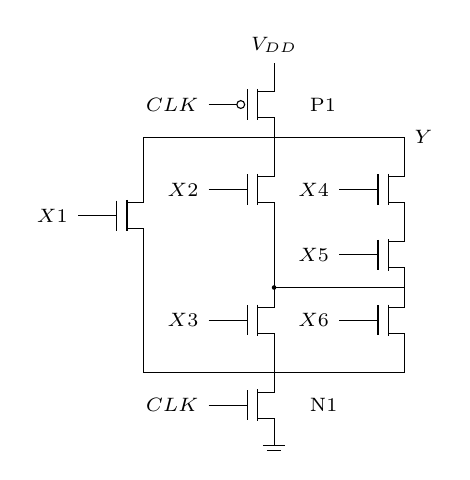
\begin{tikzpicture}[scale=.83,font=\scriptsize]
\mos{2}{5.5}{CLK}{1}\rail{2.25}{6}{V_{DD}}\node[right]at(2.65,5.5){P1};\draw(.25,5)--(4.25,5)node[right]{$Y$};
\mos{0}{3.8}{X1}{0}\draw(.25,4.3)--(.25,5);\draw(.25,3.3)--(.25,1.4);
\mos{2}{4.2}{X2}{0}\draw(2.25,4.7)--(2.25,5);\draw(2.25,3.7)--(2.25,2.7);
\mos{4}{4.2}{X4}{0}\mos{4}{3.2}{X5}{0}\draw(4.25,4.7)--(4.25,5);\draw(2.25,2.7)--(4.25,2.7);\fill(2.25,2.7)circle(1pt);
\mos{2}{2.2}{X3}{0}\mos{4}{2.2}{X6}{0}\draw(.25,1.4)--(4.25,1.4);\draw(2.25,1.7)--(2.25,1.4);\draw(4.25,1.7)--(4.25,1.4);
\mos{2}{.9}{CLK}{0}\ground{2.25}{.4}\node[right]at(2.65,.9){N1};
\end{tikzpicture}\\Figure 2: A dynamic logic circuit.\end{center}
\textbf{5. (15 points)} Figure 3 shows a combinational circuit designed with NP-domino logic. Assume that all the NMOS transistors have the same $\beta_n$ and all the PMOS transistors have the same $\beta_p$, and $\beta_n=\beta_p$. Also, $\mu_n=2\mu_p$, and the gate capacitance of the PMOS and NMOS transistors are $2C$ and $C$, respectively, and the turn-on equivalent resistance of the NMOS transistor or the PMOS transistor is $R$. Complete the following questions.
\begin{enumerate}[label=(\alph*),leftmargin=7mm]
\item Assume that the rise time $t_r$ or fall time $t_f$ of a logic gate can be estimated by the product of the output capacitance of the logic gate and the equivalent resistance of the output charge path or the output discharge path, respectively. Also, the delay of a logic gate can be calculated by $t_d=(t_r+t_f)/2$ and the drain capacitance of the transistors can be neglected. Calculate the contamination delay $t_{cd}$ and the propagation delay $t_{pd}$ of the combinational circuit in terms of $R$ and $C$. (10 points)
\item Assume that $V_{dd}$ of the combinational circuit is 1.8 V and the threshold voltage of the PMOS transistor is $|V_{tp}|=.6$ V. Also, the capacitance of nodes $x$, $y$, and $z$ are .4 pf, .8 pf, and 2 pf, respectively. Can the combinational circuit be operated correctly? Explain your answer. (5 points)
\end{enumerate}
\begin{center}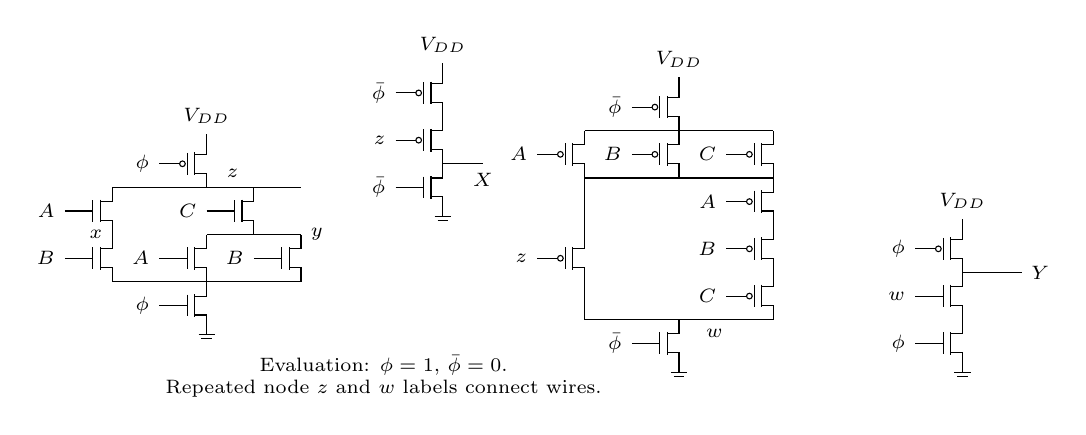
\begin{tikzpicture}[scale=.60,font=\scriptsize]
\mos{2}{5.8}{\phi}{1}\rail{2.25}{6.3}{V_{DD}}\draw(.25,5.3)--(4.25,5.3);\node[above]at(2.8,5.3){$z$};
\mos{0}{4.8}{A}{0}\mos{0}{3.8}{B}{0}\node[left]at(.25,4.3){$x$};\mos{3}{4.8}{C}{0}\draw(3.25,4.3)--(4.25,4.3);\mos{2}{3.8}{A}{0}\mos{4}{3.8}{B}{0}\draw(2.25,4.3)--(3.25,4.3);\node[right]at(4.25,4.3){$y$};\draw(.25,3.3)--(4.25,3.3);\mos{2}{2.8}{\phi}{0}\ground{2.25}{2.3}
\mos{7}{7.3}{\bar\phi}{1}\rail{7.25}{7.8}{V_{DD}}\mos{7}{6.3}{z}{1}\mos{7}{5.3}{\bar\phi}{0}\ground{7.25}{4.8}\draw(7.25,5.8)--(8.1,5.8)node[below]{$X$};
\mos{12}{7}{\bar\phi}{1}\rail{12.25}{7.5}{V_{DD}}\draw(10.25,6.5)--(14.25,6.5);\mos{10}{6}{A}{1}\mos{12}{6}{B}{1}\mos{14}{6}{C}{1}\draw(10.25,5.5)--(14.25,5.5);
\mos{10}{3.8}{z}{1}\draw(10.25,4.3)--(10.25,5.5);\draw(10.25,3.3)--(10.25,2.5)--(14.25,2.5);
\mos{14}{5}{A}{1}\mos{14}{4}{B}{1}\mos{14}{3}{C}{1}\mos{12}{2}{\bar\phi}{0}\ground{12.25}{1.5}\node[below]at(13,2.5){$w$};
\mos{18}{4}{\phi}{1}\rail{18.25}{4.5}{V_{DD}}\mos{18}{3}{w}{0}\mos{18}{2}{\phi}{0}\ground{18.25}{1.5}\draw(18.25,3.5)--(19.5,3.5)node[right]{$Y$};
\node[align=center]at(6,1.3){Evaluation: $\phi=1$, $\bar\phi=0$.\\Repeated node $z$ and $w$ labels connect wires.};\end{tikzpicture}\\Figure 3: NP-domino logic.\end{center}
\newpage
\textbf{6. (10 points)} Figure 4(a) shows a pipelined circuit. Assume that your boss asks you to design the circuit such that the circuit can be operated at 100 MHz. Also, the clock-to-Q propagation delay ($t_{pcq}$), the clock-to-Q contamination delay ($t_{ccq}$), the setup time ($t_{setup}$), and the hold time ($t_{hold}$) of registers R1, R2, and R3 are .8 ns, .4 ns, 1.6 ns, and 1.2 ns, respectively. Complete the following questions.
\begin{enumerate}[label=(\alph*),leftmargin=7mm]
\item If the clock skew of CLK is .1 ns, determine the maximum delay of the combinational circuit. (5 points)
\item If the delay of the interconnection between R2 and R3 is .2 ns and the delay of the buffer shown in Figure 4(b) is .3 ns, then how do you design the pipeline circuit such that it can be operated correctly? Draw the modified pipelined circuit. (5 points)
\end{enumerate}
\begin{center}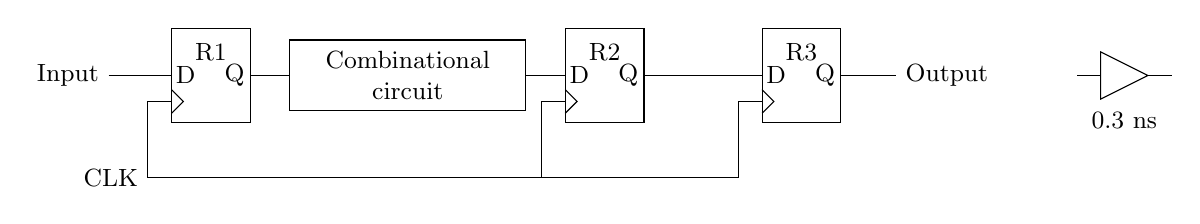
\begin{tikzpicture}[font=\small]
\foreach\x/\r in{0/R1,5/R2,7.5/R3}{\draw(\x,0)rectangle(\x+1,1.2);\node at(\x+.5,.9){\r};\node at(\x+.18,.6){D};\node at(\x+.8,.6){Q};\draw(\x,.12)--(\x+.15,.27)--(\x,.42);\draw(\x,.27)--(\x-.3,.27)--(\x-.3,-.7);}
\draw(-.8,.6)--(0,.6)node[pos=0,left]{Input};\draw(1,.6)--(1.5,.6);\draw(1.5,.15)rectangle(4.5,1.05);\node[align=center]at(3,.6){Combinational\\circuit};\draw(4.5,.6)--(5,.6);\draw(6,.6)--(7.5,.6);\draw(8.5,.6)--(9.2,.6)node[right]{Output};\draw(-.3,-.7)--(7.2,-.7);\node[left]at(-.3,-.7){CLK};
\begin{scope}[xshift=11.8cm]\draw(0,.3)--(0,.9)--(.6,.6)--cycle;\draw(-.3,.6)--(0,.6) (.6,.6)--(.9,.6);\node[below]at(.3,.25){0.3 ns};\end{scope}
\end{tikzpicture}\\Figure 4: (a) Pipeline (b) buffer.\end{center}
\textbf{7. (15 points)} Figure 5 shows the symbolic layout of a circuit. Draw its transistor-level schematic.
\begin{center}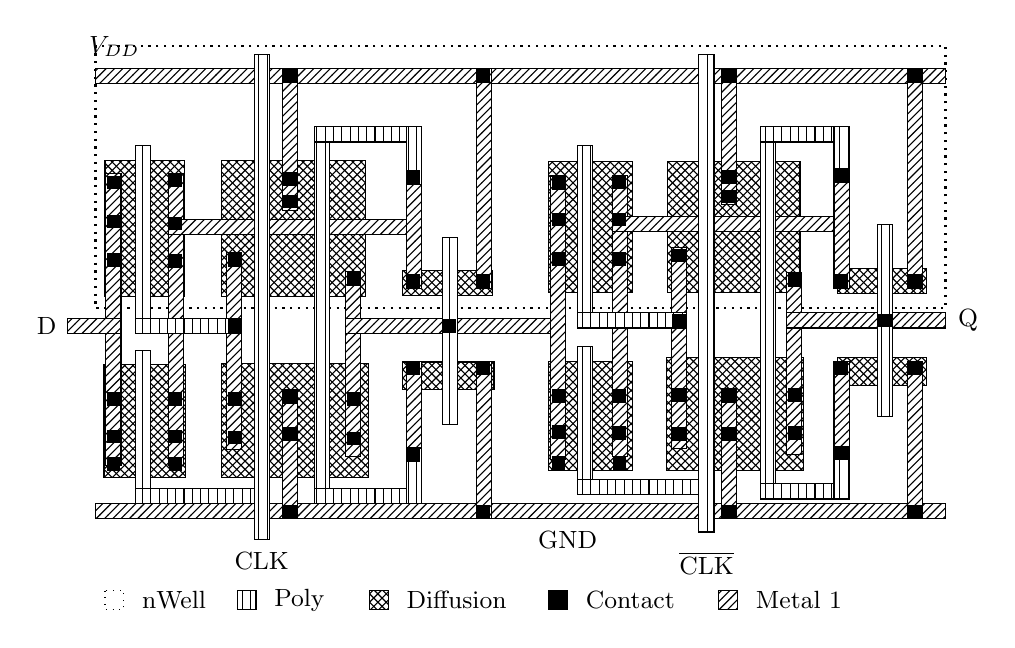
\begin{tikzpicture}[x=.012cm,y=-.012cm,font=\small]
\tikzset{lm/.style={preaction={fill=white},pattern=north east lines,pattern color=black},ld/.style={preaction={fill=white},pattern=crosshatch,pattern color=black},lp/.style={preaction={fill=white},pattern=vertical lines,pattern color=black}}
\draw[dotted,thick](400,108)rectangle(1300,386);
\draw[ld](410,230)rectangle(494,374);
\draw[ld](533,230)rectangle(686,374);
\draw[ld](725,346)rectangle(820,373);
\draw[ld](880,231)rectangle(969,369);
\draw[ld](1006,231)rectangle(1146,369);
\draw[ld](1186,344)rectangle(1280,370);
\draw[ld](409,446)rectangle(495,565);
\draw[ld](533,445)rectangle(689,565);
\draw[ld](725,443)rectangle(822,472);
\draw[ld](880,442)rectangle(969,558);
\draw[ld](1005,438)rectangle(1150,558);
\draw[ld](1186,438)rectangle(1280,468);
\draw[lm](400,132.0)rectangle(1300,148.0);
\draw[lm](400,593.0)rectangle(1300,609.0);
\draw[lm](411.0,243.0)rectangle(427.0,553.0);
\draw[lm](477.0,243.0)rectangle(493.0,553.0);
\draw[lm](477.0,292.0)rectangle(745.0,308.0);
\draw[lm](729.0,239.0)rectangle(745.0,365.0);
\draw[lm](539.0,327.0)rectangle(555.0,536.0);
\draw[lm](598.0,132.0)rectangle(614.0,283.0);
\draw[lm](598.0,472.0)rectangle(614.0,609.0);
\draw[lm](665.0,347.0)rectangle(681.0,543.0);
\draw[lm](665.0,397.0)rectangle(898.0,413.0);
\draw[lm](803.0,132.0)rectangle(819.0,365.0);
\draw[lm](803.0,442.0)rectangle(819.0,609.0);
\draw[lm](729.0,442.0)rectangle(745.0,550.0);
\draw[lm](882.0,246.0)rectangle(898.0,546.0);
\draw[lm](947.0,245.0)rectangle(963.0,543.0);
\draw[lm](947.0,289.0)rectangle(1198.0,305.0);
\draw[lm](1182.0,237.0)rectangle(1198.0,365.0);
\draw[lm](1010.0,322.0)rectangle(1026.0,535.0);
\draw[lm](1063.0,132.0)rectangle(1079.0,276.0);
\draw[lm](1063.0,471.0)rectangle(1079.0,609.0);
\draw[lm](1132.0,348.0)rectangle(1148.0,541.0);
\draw[lm](1132.0,391.0)rectangle(1300,407.0);
\draw[lm](1260.0,132.0)rectangle(1276.0,365.0);
\draw[lm](1260.0,442.0)rectangle(1276.0,609.0);
\draw[lm](1182.0,442.0)rectangle(1198.0,548.0);
\draw[lp](442.0,214.0)rectangle(458.0,413.0);
\draw[lp](442.0,397.0)rectangle(555.0,413.0);
\draw[lp](442.0,431.0)rectangle(458.0,593.0);
\draw[lp](442.0,577.0)rectangle(584.0,593.0);
\draw[lp](568.0,117.0)rectangle(584.0,631.0);
\draw[lp](632.0,194.0)rectangle(648.0,593.0);
\draw[lp](632.0,194.0)rectangle(745.0,210.0);
\draw[lp](729.0,194.0)rectangle(745.0,255.0);
\draw[lp](632.0,577.0)rectangle(745.0,593.0);
\draw[lp](729.0,534.0)rectangle(745.0,593.0);
\draw[lp](767.0,311.0)rectangle(783.0,509.0);
\draw[lp](910.0,214.0)rectangle(926.0,407.0);
\draw[lp](910.0,391.0)rectangle(1026.0,407.0);
\draw[lp](910.0,427.0)rectangle(926.0,583.0);
\draw[lp](910.0,567.0)rectangle(1055.0,583.0);
\draw[lp](1039.0,117.0)rectangle(1055.0,623.0);
\draw[lp](1104.0,194.0)rectangle(1120.0,588.0);
\draw[lp](1104.0,194.0)rectangle(1198.0,210.0);
\draw[lp](1182.0,194.0)rectangle(1198.0,253.0);
\draw[lp](1104.0,572.0)rectangle(1198.0,588.0);
\draw[lp](1182.0,532.0)rectangle(1198.0,588.0);
\draw[lp](1228.0,297.0)rectangle(1244.0,501.0);
\draw[fill=black](540.5,398.5)rectangle(553.5,411.5);
\draw[fill=black](730.5,240.5)rectangle(743.5,253.5);
\draw[fill=black](730.5,535.5)rectangle(743.5,548.5);
\draw[fill=black](768.5,398.5)rectangle(781.5,411.5);
\draw[fill=black](1011.5,392.5)rectangle(1024.5,405.5);
\draw[fill=black](1183.5,238.5)rectangle(1196.5,251.5);
\draw[fill=black](1183.5,533.5)rectangle(1196.5,546.5);
\draw[fill=black](1229.5,392.5)rectangle(1242.5,405.5);
\draw[fill=black](599.5,133.5)rectangle(612.5,146.5);
\draw[fill=black](599.5,594.5)rectangle(612.5,607.5);
\draw[fill=black](804.5,133.5)rectangle(817.5,146.5);
\draw[fill=black](804.5,594.5)rectangle(817.5,607.5);
\draw[fill=black](1064.5,133.5)rectangle(1077.5,146.5);
\draw[fill=black](1064.5,594.5)rectangle(1077.5,607.5);
\draw[fill=black](1261.5,133.5)rectangle(1274.5,146.5);
\draw[fill=black](1261.5,594.5)rectangle(1274.5,607.5);
\draw[fill=black](412.5,246.5)rectangle(425.5,259.5);
\draw[fill=black](412.5,287.5)rectangle(425.5,300.5);
\draw[fill=black](412.5,328.5)rectangle(425.5,341.5);
\draw[fill=black](478.5,244.5)rectangle(491.5,257.5);
\draw[fill=black](478.5,289.5)rectangle(491.5,302.5);
\draw[fill=black](478.5,329.5)rectangle(491.5,342.5);
\draw[fill=black](540.5,328.5)rectangle(553.5,341.5);
\draw[fill=black](599.5,242.5)rectangle(612.5,255.5);
\draw[fill=black](599.5,266.5)rectangle(612.5,279.5);
\draw[fill=black](666.5,348.5)rectangle(679.5,361.5);
\draw[fill=black](730.5,350.5)rectangle(743.5,363.5);
\draw[fill=black](804.5,350.5)rectangle(817.5,363.5);
\draw[fill=black](883.5,247.5)rectangle(896.5,260.5);
\draw[fill=black](883.5,285.5)rectangle(896.5,298.5);
\draw[fill=black](883.5,327.5)rectangle(896.5,340.5);
\draw[fill=black](948.5,246.5)rectangle(961.5,259.5);
\draw[fill=black](948.5,285.5)rectangle(961.5,298.5);
\draw[fill=black](948.5,327.5)rectangle(961.5,340.5);
\draw[fill=black](1011.5,323.5)rectangle(1024.5,336.5);
\draw[fill=black](1064.5,240.5)rectangle(1077.5,253.5);
\draw[fill=black](1064.5,261.5)rectangle(1077.5,274.5);
\draw[fill=black](1133.5,349.5)rectangle(1146.5,362.5);
\draw[fill=black](1183.5,350.5)rectangle(1196.5,363.5);
\draw[fill=black](1261.5,350.5)rectangle(1274.5,363.5);
\draw[fill=black](412.5,475.5)rectangle(425.5,488.5);
\draw[fill=black](412.5,515.5)rectangle(425.5,528.5);
\draw[fill=black](412.5,544.5)rectangle(425.5,557.5);
\draw[fill=black](478.5,475.5)rectangle(491.5,488.5);
\draw[fill=black](478.5,515.5)rectangle(491.5,528.5);
\draw[fill=black](478.5,544.5)rectangle(491.5,557.5);
\draw[fill=black](540.5,475.5)rectangle(553.5,488.5);
\draw[fill=black](540.5,516.5)rectangle(553.5,529.5);
\draw[fill=black](599.5,473.5)rectangle(612.5,486.5);
\draw[fill=black](599.5,512.5)rectangle(612.5,525.5);
\draw[fill=black](666.5,475.5)rectangle(679.5,488.5);
\draw[fill=black](666.5,517.5)rectangle(679.5,530.5);
\draw[fill=black](730.5,443.5)rectangle(743.5,456.5);
\draw[fill=black](804.5,443.5)rectangle(817.5,456.5);
\draw[fill=black](883.5,472.5)rectangle(896.5,485.5);
\draw[fill=black](883.5,510.5)rectangle(896.5,523.5);
\draw[fill=black](883.5,543.5)rectangle(896.5,556.5);
\draw[fill=black](948.5,472.5)rectangle(961.5,485.5);
\draw[fill=black](948.5,511.5)rectangle(961.5,524.5);
\draw[fill=black](948.5,543.5)rectangle(961.5,556.5);
\draw[fill=black](1011.5,471.5)rectangle(1024.5,484.5);
\draw[fill=black](1011.5,512.5)rectangle(1024.5,525.5);
\draw[fill=black](1064.5,472.5)rectangle(1077.5,485.5);
\draw[fill=black](1064.5,512.5)rectangle(1077.5,525.5);
\draw[fill=black](1133.5,471.5)rectangle(1146.5,484.5);
\draw[fill=black](1133.5,511.5)rectangle(1146.5,524.5);
\draw[fill=black](1183.5,443.5)rectangle(1196.5,456.5);
\draw[fill=black](1261.5,443.5)rectangle(1274.5,456.5);
\node[above]at(420,130){$V_{DD}$};\node[below]at(900,612){GND};\draw[lm](370,397)rectangle(427,413);
\node[left]at(369,405){D};\node[right]at(1303,399){Q};
\node[below]at(576,634){CLK};\node[below]at(1047,634){$\overline{\mathrm{CLK}}$};
\draw[dotted](410,685)rectangle(430,705);\node[right]at(439,695){nWell};
\draw[lp](550,685)rectangle(570,705);\node[right]at(579,695){Poly};
\draw[ld](690,685)rectangle(710,705);\node[right]at(719,695){Diffusion};
\draw[fill=black](880,685)rectangle(900,705);\node[right]at(909,695){Contact};
\draw[lm](1060,685)rectangle(1080,705);\node[right]at(1089,695){Metal 1};
\end{tikzpicture}\\[2mm]\small Geometry normalized; all eight physical gate columns and contacts retained.\end{center}\begin{center}Figure 5: Symbolic layout.\end{center}
\textbf{8. (15 points)} Figure 6 shows the Schmitt CMOS circuit and its voltage transfer curve. Assume that the supply voltage $V_{dd}=1.8$ V and the threshold voltage of the NMOS transistors is $V_{tn}=.6$ V. Your boss asks you to design the Schmitt CMOS circuit such that its $V_T^+=1.2$ V. Please derive the ratio of $\beta_{N1}$ to $\beta_{N3}$.
\begin{center}\begin{tikzpicture}[scale=.82,font=\scriptsize]
\mos{1}{4.5}{}{1}\mos{1}{3.5}{}{1}\mos{1}{2}{}{0}\mos{1}{1}{}{0}\rail{1.25}{5}{1.8\,V}\ground{1.25}{.5}
\foreach\y/\name in{4.5/P1,3.5/P2,2/N2,1/N1}{\node[right]at(1.5,\y){\name};}
\draw(1.25,2.5)--(1.25,3);\draw(1.25,2.75)--(5,2.75)node[right]{$V_{out}$};\draw(-.8,1)--(-.8,4.5);\foreach\y in{1,2,3.5,4.5}{\draw(-.8,\y)--(.25,\y);}\node[left]at(-.8,2.75){$V_{in}$};
\hmos{3.2}{4.25}{P3}{1}\draw(1.25,4)--(2.7,4);\draw(3.7,4)--(4.2,4);\ground{4.2}{4}\draw(3.2,5)--(4.6,5)--(4.6,2.75);
\hmos{3.2}{1.75}{N3}{0}\draw(1.25,1.5)--(2.7,1.5);\draw(3.7,1.5)--(4.2,1.5);\rail{4.2}{1.5}{1.8\,V}\draw(3.2,2.5)--(3.2,2.75);\fill(3.2,2.75)circle(1pt);
\begin{scope}[xshift=7cm]\draw[->](0,0)--(4.5,0)node[right]{$V_{in}$};\draw[->](0,0)--(0,3.5)node[above]{$V_{out}$};\draw plot[smooth]coordinates{(0,3)(1,3)(1.4,2.8)(1.65,1.5)(1.9,.2)(3.5,0)};\draw plot[smooth]coordinates{(0,3)(2,3)(2.8,2.8)(3,1.5)(3.2,.2)(3.7,0)};\draw[->](.5,3)--(1,3);\draw[->](3,1.8)--(3,1.2);\draw[->](1.65,1.2)--(1.65,1.8);\draw[->](2.8,.01)--(2.3,.01);\draw[dashed](1.65,0)--(1.65,1.5) (3,0)--(3,1.5);\node[below]at(1.65,0){$V_T^-$};\node[below]at(3,0){$V_T^+=1.2$};\end{scope}
\end{tikzpicture}\\Figure 6: Schmitt circuit and qualitative VTC.\end{center}\vfill\small All source values and connections preserved. The reconstruction supplies editable question text and figures. Drawn dimensions and qualitative VTC spacing are normalized for readability.\end{document}